88. $y=\cfrac{4-x^2}{x+2}-1=\cfrac{(2-x)(2+x)}{x+2}-1=\begin{cases} 1-x,\\ x\neq-2.\end{cases}$\\
\begin{figure}[ht!]
\center{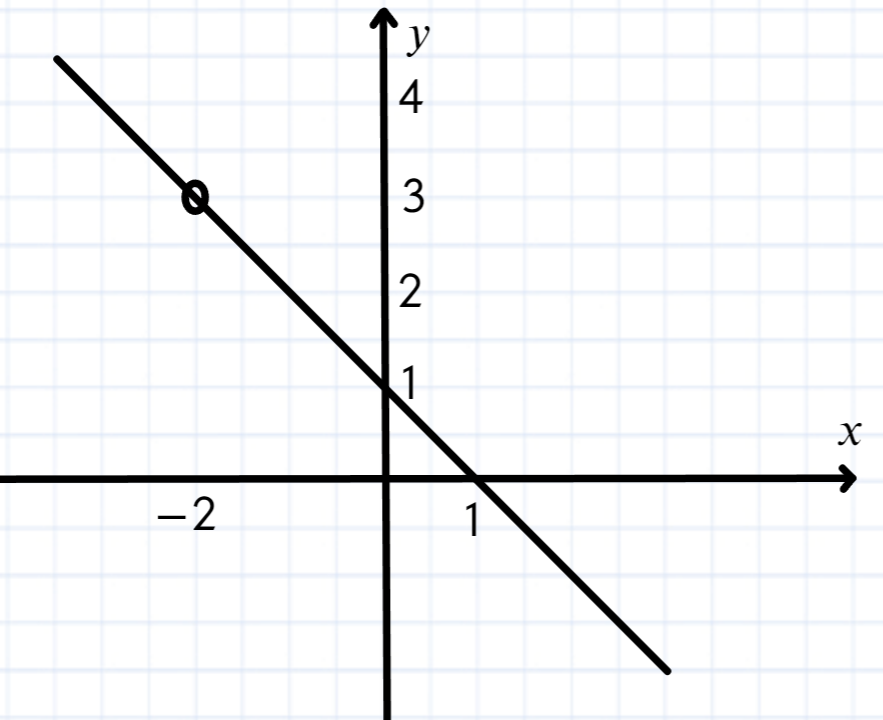
\includegraphics[scale=0.35]{gr7-88.png}}
\end{figure}\\
По графику определим подходящие значения 1, 2 и 4.\\
